\section{The DisasterClaw platform}
\label{sec:platform}
\subsection{Design objectives and system architecture}
DisasterClaw is an imagery-based simulation and evaluation framework for single-UAV disaster inspection. Its purpose is to turn georeferenced disaster records into closed-loop episodes in which an agent changes its map position or observation footprint, receives a new image, and is scored on a disaster task. The implementation has four connected layers (Fig.~\ref{fig:overview}): a task interface, a disaster-response agent, a simulated geospatial world, and an instrumentation layer. The operator-facing path uses a React/Vite console connected to a Flask/Socket.IO service. Quantitative experiments use a headless runner that calls the same environment and controller modules without rendering the user interface.

\begin{figure}[htbp]
\centering
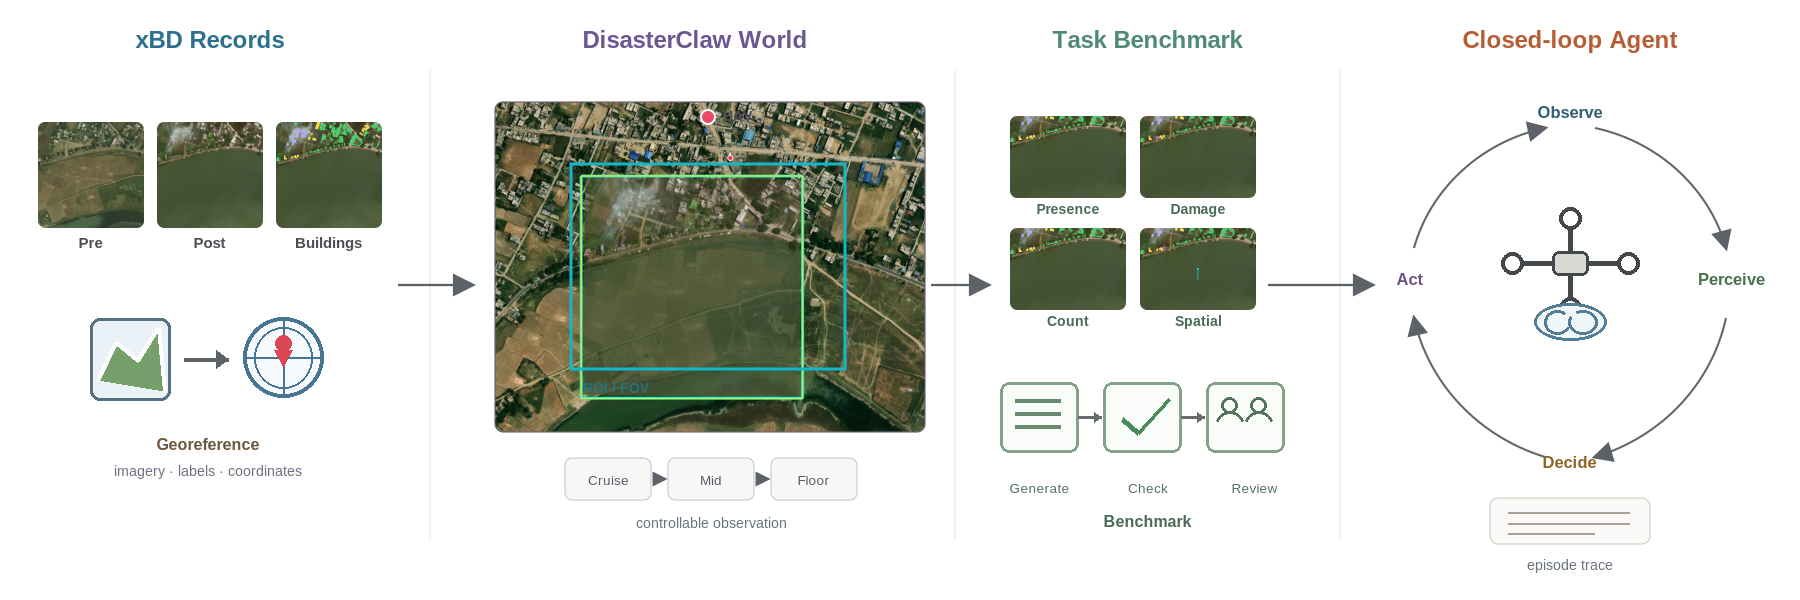
\includegraphics[width=\linewidth]{figure-paper/Fig_DisasterClaw_Refined_NoOverlap.png}
\caption{Data-to-episode workflow in DisasterClaw. Paired xBD imagery and building annotations provide a geographic scene and reference evidence; map anchoring makes observations depend on vehicle state; task generation, checks, and review produce a frozen benchmark; the platform records closed-loop inspection episodes. Image panels illustrate these stages rather than documenting one final-test trajectory.}
\label{fig:overview}
\end{figure}

Table~\ref{tab:platform} states what each layer implements and the boundary attached to it. This distinction is central to the intended use of the platform. Its geospatial state and image renderer support controlled observation studies; they do not reproduce the complete physics of an aircraft or camera.

\begin{table}[htbp]
\centering\footnotesize
\caption{Implemented DisasterClaw capabilities and their evaluation boundaries.}
\label{tab:platform}
\begin{tabularx}{\linewidth}{@{}>{\raggedright\arraybackslash}p{2.25cm}>{\raggedright\arraybackslash}X>{\raggedright\arraybackslash}X@{}}
\toprule
Capability & Implemented function & Boundary in this study \\
\midrule
Scene & Georeferenced pre-/post-disaster tiles, building annotations, map anchors, target ROIs, and contextual basemap & Three evaluated events and 44 ROIs; incomplete source archive and no global coverage claim \\
Observation & Nadir fixed-FOV crop and resampling at three footprint widths; paired archival and current-image channels & Orthographic imagery; no new viewpoint, acquisition time, or detail below the assumed 0.5 m/pixel source scale \\
Vehicle and actions & Geographic and local position, altitude, heading, speed, task state, straight-line motion, centering, descent, hover, marking, and reporting & One UAV with simplified kinematics; no six-degree-of-freedom dynamics, wind, collision, communication, or battery model \\
Perception and models & Building localization and binary no-damage/damaged evidence, geographic cross-view evidence memory, task-specific spatial summaries, and Qwen answer generation & Fixed ChangeOS backend with prior xBD exposure; fixed Qwen2.5-VL-7B-Instruct answer model; no claim of event-disjoint perception generalization \\
Tasks & Operator instructions, damage/presence/count/spatial questions, and archived language-guided navigation instructions & Task-scoped simulation; no claim of unrestricted natural-language or open-world competence \\
Logging and evaluation & Interactive monitoring, headless episodes, paired task IDs, intermediate evidence, actions, budgets, answers, and terminal scores & All 3,360 final online episodes are covered by local shard-level consistency audits; complete public release packaging remains pending \\
Physical boundary & Map-anchored scene transitions and a controlled observation ladder & No photorealistic sensor synthesis, aircraft certification model, hardware-in-the-loop result, or physical-flight validation \\
\bottomrule
\end{tabularx}

\end{table}

The design has three objectives: retain the geographic relationship between source imagery and inspection targets, expose a controllable observation through a common agent interface, and preserve the evidence needed to reconstruct task outcomes. The benchmark is constructed from the same registered source records, but its reference annotations are kept separate from agent observations. This separates world construction, answer construction, and policy execution.

\subsection{Map-anchored disaster-world construction}
The scene layer reads paired pre- and post-disaster tiles, building polygons, damage labels, and geographic metadata derived from xBD. Pixel-to-geographic and geographic-to-pixel affine transforms place each image on its recorded ground footprint. When a tile becomes active, its center defines the local world anchor. Robot, target, and report coordinates remain available as latitude, longitude, and altitude, while local north and east offsets are recomputed relative to that anchor.

The interactive map can place the active disaster image over a satellite or street basemap, display the tile boundary, and color annotated buildings for operator reference. These annotation overlays are not passed to the evaluated agent as visual input. In rendered observations, georeferenced disaster tiles supply task evidence and the surrounding basemap supplies spatial context when a wider footprint extends beyond the available disaster tile. Reference answers and building-level scores remain restricted to the annotated target ROI, so contextual background is not treated as disaster ground truth.

The evaluated scene population contains three disaster events and 44 target ROIs. This is the experimental subset, not a claim that the software can reproduce every disaster represented by the source dataset. Missing tiles, sparse geographic coverage, affine-registration error, and differences in acquisition date all constrain the resulting environment.

\begin{figure}[htbp]
\centering
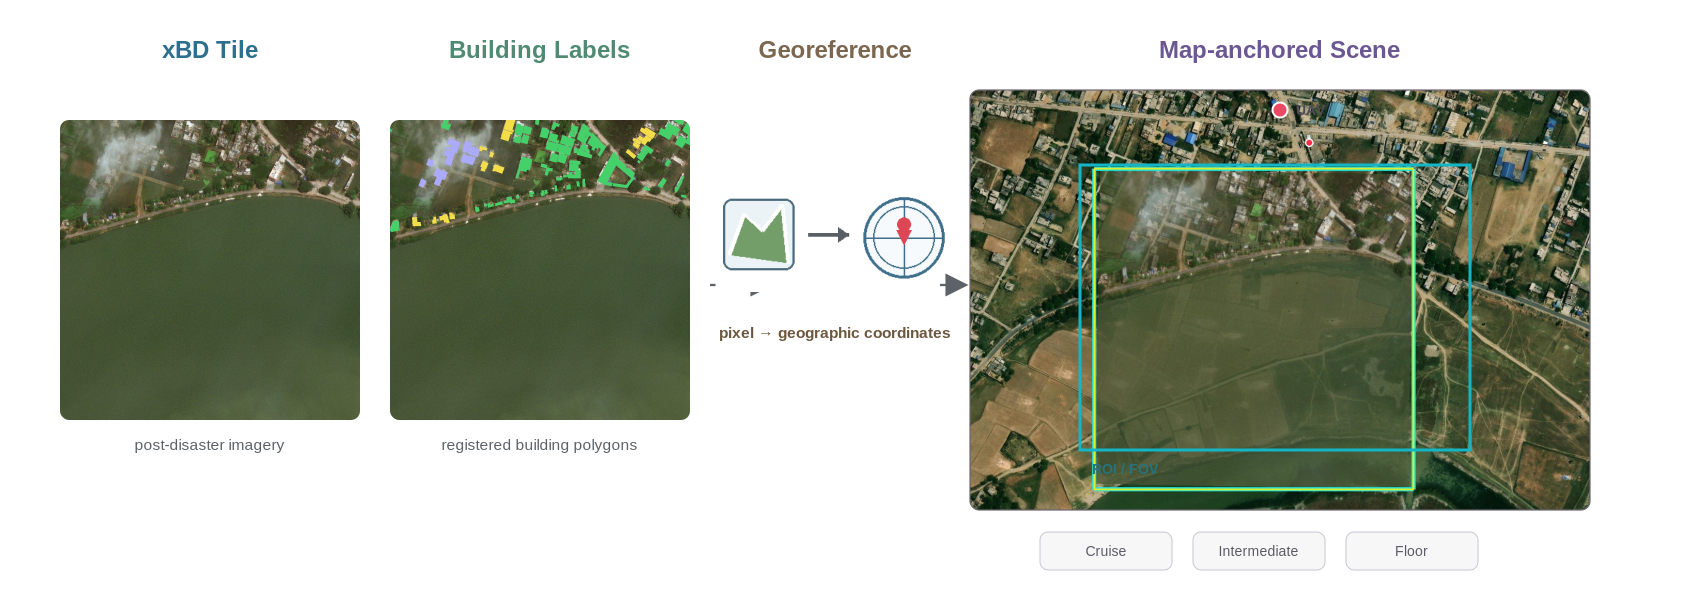
\includegraphics[width=\linewidth]{figure-paper/Fig2_MapAnchored_Integration.png}
\caption{Geographic embedding of disaster records. Image footprints and building polygons are placed in a shared map coordinate system, allowing the environment to associate observations and target locations with geographic state. The supplied visualization illustrates registration and overlays; its colors and markers are not a verified final-task answer key. Basemap context outside the annotated ROI does not supply disaster ground truth.}
\label{fig:map-anchored}
\end{figure}

\subsection{Controllable observation model}
The simulated sensor is nadir-facing, with horizontal field of view $\theta$ and fixed output width $W$. For vehicle height $h$, the ground-footprint width $L$ and effective ground sampling distance $g$ are
\begin{equation}
 L(h)=2h\tan(\theta/2),\qquad g(h)=\frac{L(h)}{W}.
 \label{eq:geometry}
\end{equation}
We use $\theta=60^\circ$, $W=1024$, and an assumed source scale of $0.5$ m/pixel. A $1024$-pixel source tile therefore spans 512 m. Footprints of three, two, and one tile widths define cruise, intermediate, and floor states at approximately 1330.2, 886.8, and 443.4 m, with effective GSDs of 1.5, 1.0, and 0.5 m/pixel (Fig.~\ref{fig:ladder}). The heights are derived parameters of this camera abstraction; they are not measured flight altitudes from the source imagery.

\begin{figure}[htbp]
\centering
\resizebox{\linewidth}{!}{\begin{tikzpicture}[
  font=\footnotesize,
  >=Latex,
  view/.style={draw=black!65,minimum width=3.35cm,minimum height=2.45cm,inner sep=0pt},
  note/.style={align=center,text width=3.45cm,font=\scriptsize}
]
% Source mosaic and nested ground footprints.
\begin{scope}[shift={(3.85,3.55)}]
  \draw[fill=gray!6,draw=black!65] (0,0) rectangle (4.0,3.55);
  \foreach \x in {1.333,2.667}{\draw[gray!42] (\x,0)--(\x,3.55);}
  \foreach \y in {1.183,2.367}{\draw[gray!42] (0,\y)--(4,\y);}
  \draw[line width=4pt,white] (-.05,.58)--(4.05,2.72);
  \draw[line width=.8pt,gray!55] (-.05,.58)--(4.05,2.72);
  \draw[line width=3.2pt,white] (3.05,-.05)--(1.08,3.60);
  \draw[line width=.7pt,gray!55] (3.05,-.05)--(1.08,3.60);
  \foreach \p in {(.45,2.75),(.82,2.92),(3.02,2.91),(3.40,3.08),(3.00,.42),(3.38,.56),(.43,.34),(.80,.49)}{
    \draw[fill=gray!42,draw=gray!65] \p ++(-.14,-.09) rectangle ++(.28,.18);
  }
  \fill[red!75] (2.02,1.79) circle (2.3pt);
  \node[red!65!black,anchor=south west] at (2.08,1.84) {target ROI};
  \draw[line width=1.4pt,blue!65!black] (.17,.15) rectangle (3.83,3.40);
  \draw[line width=1.4pt,orange!85!black] (.73,.65) rectangle (3.27,2.90);
  \draw[line width=1.4pt,green!55!black] (1.34,1.18) rectangle (2.70,2.39);
  \node[anchor=north] at (2,-.15) {map-anchored disaster scene};
\end{scope}

\node[anchor=west,align=left,font=\scriptsize] at (8.30,6.40) {\textcolor{blue!65!black}{\rule{9pt}{2pt}} cruise: $3\!\times\!3$ tiles};
\node[anchor=west,align=left,font=\scriptsize] at (8.30,5.62) {\textcolor{orange!85!black}{\rule{9pt}{2pt}} intermediate: $2\!\times\!2$};
\node[anchor=west,align=left,font=\scriptsize] at (8.30,4.84) {\textcolor{green!55!black}{\rule{9pt}{2pt}} floor: $1\!\times\!1$ tile};

% Three observations have the same output size.
\begin{scope}[shift={(0,0.45)}]
  \node[view,anchor=south west] at (0,0) {};
  \clip (0,0) rectangle (3.35,2.45);
  \draw[line width=3.5pt,gray!30] (-.2,.25)--(3.55,2.22);
  \draw[line width=2.8pt,gray!30] (2.95,-.15)--(.62,2.62);
  \foreach \p in {(.35,1.91),(.73,2.06),(2.55,2.02),(2.91,2.16),(2.64,.36),(.52,.40)}{
    \draw[fill=gray!38,draw=gray!60] \p ++(-.14,-.09) rectangle ++(.28,.18);
  }
  \draw[very thick,red!75] (1.12,.71) rectangle (2.23,1.82);
  \node[fill=blue!65!black,text=white,rounded corners=1pt,inner sep=2pt] at (1.675,2.21) {cruise};
\end{scope}
\node[note,anchor=north] at (1.675,.34) {$h\approx1330.2$ m; 1.5 m/px\\target occupies $\approx1/3$ width};

\begin{scope}[shift={(4.08,0.45)}]
  \node[view,anchor=south west] at (0,0) {};
  \clip (0,0) rectangle (3.35,2.45);
  \draw[line width=3.5pt,gray!30] (-.25,.12)--(3.6,2.36);
  \draw[line width=2.8pt,gray!30] (3.05,-.18)--(.40,2.63);
  \foreach \p in {(.28,1.96),(2.84,2.09),(2.87,.30),(.40,.31)}{
    \draw[fill=gray!38,draw=gray!60] \p ++(-.16,-.10) rectangle ++(.32,.20);
  }
  \draw[very thick,red!75] (.84,.48) rectangle (2.51,2.15);
  \node[fill=orange!85!black,text=white,rounded corners=1pt,inner sep=2pt] at (1.675,2.21) {intermediate};
\end{scope}
\node[note,anchor=north] at (5.755,.34) {$h\approx886.8$ m; 1.0 m/px\\target occupies $\approx1/2$ width};

\begin{scope}[shift={(8.16,0.45)}]
  \node[view,anchor=south west] at (0,0) {};
  \clip (0,0) rectangle (3.35,2.45);
  \draw[line width=3.5pt,gray!30] (-.35,-.02)--(3.7,2.54);
  \draw[line width=2.8pt,gray!30] (3.18,-.23)--(.12,2.67);
  \draw[very thick,red!75] (.30,.20) rectangle (3.05,2.25);
  \node[fill=green!55!black,text=white,rounded corners=1pt,inner sep=2pt] at (1.675,2.21) {floor};
\end{scope}
\node[note,anchor=north] at (9.835,.34) {$h\approx443.4$ m; 0.5 m/px\\source-resolution floor};

\draw[->,thick,blue!65!black] (4.20,4.05) to[bend right=18] (1.68,3.02);
\draw[->,thick,orange!85!black] (5.84,4.05) -- (5.76,3.02);
\draw[->,thick,green!55!black] (7.50,4.05) to[bend left=18] (9.84,3.02);
\end{tikzpicture}
}
\caption{Observation construction from one georeferenced scene. Each state is rendered to $1024\times1024$ pixels. Descending narrows the ground footprint and assigns more existing source pixels to the target ROI; the floor state reaches, but cannot exceed, the assumed source resolution.}
\label{fig:ladder}
\end{figure}

For paired damage perception, the post-disaster channel is sampled at the current footprint and fixed output size. The corresponding pre-disaster window is retained at the assumed source scale before the pair is brought to the detector input geometry. This represents access to an archival reference and a controllable current observation. It also means the two channels undergo different resampling. The platform records this choice because it can contribute to any observed view response.

Changing height only crops and resamples existing orthographic imagery. The renderer does not create sub-source detail, oblique views, three-dimensional parallax, self-occlusion, atmospheric effects, motion blur, or a new acquisition time. At the floor, further descent cannot add information under the adopted source model.

\subsection{Agent--environment interaction interface}
The world model stores a single UAV with geographic position, altitude, heading, speed, flight status, and task state. It also stores targets, reports, the active disaster tile, map bounds, and timestamps. Motion is implemented by straight-line interpolation in a locally anchored horizontal frame. A position update is converted between geographic coordinates and local north--east offsets, and altitude is recorded as the vertical state.

The task planner and closed-loop agent share a finite set of environment tools: fly to a geographic coordinate, move by a relative horizontal or vertical offset, hover, run disaster detection, mark a target, and produce a report. The inspection controller additionally uses answer, abstain, and stop as episode decisions. A reobservation maps to one or more movement primitives, such as centering on evidence and descending by one camera-ladder state, followed by a new render and perception pass.

This action model supports repeatable studies of where the sensor is pointed and how often another observation is requested. It omits rigid-body attitude dynamics, acceleration limits, wind, terrain following, collision checking, communications, and battery discharge. Executed action count is therefore the principal online cost in this paper. Any time estimate obtained from configured speeds remains a simulator quantity rather than measured endurance.

\subsection{Instrumentation and benchmark execution}
The console exposes disaster selection, a georeferenced situation map, manual flight controls, language-task submission, perception displays, agent state, and event logs. An operator can activate a disaster tile, select a target location, issue an inspection task, observe the planned or closed-loop actions, and inspect the returned damage evidence. The operator console supports qualitative inspection of the same scene state, perception evidence, decisions, actions, budgets, and event logs used by the headless benchmark. The interface is intended for monitoring and diagnosis; all quantitative results in this study are produced by the frozen headless protocol.

The headless benchmark initializes a question and vehicle state, invokes the same observation and action modules, and writes the evolving answer, evidence, controller decision, movement, budget, and terminal outcome. Frozen question identifiers allow policies to be compared on paired tasks. The implementation also supports a fixed-view mode that holds the environment state constant while repeating answer generation. The final benchmark binds generation seeds to question, repeat, step, and call role, making environmental changes and subsequent generation calls separately traceable. Policies may still make different numbers of later calls, so whole-policy comparisons are not pure action-only effects.

\begin{figure}[htbp]
\centering
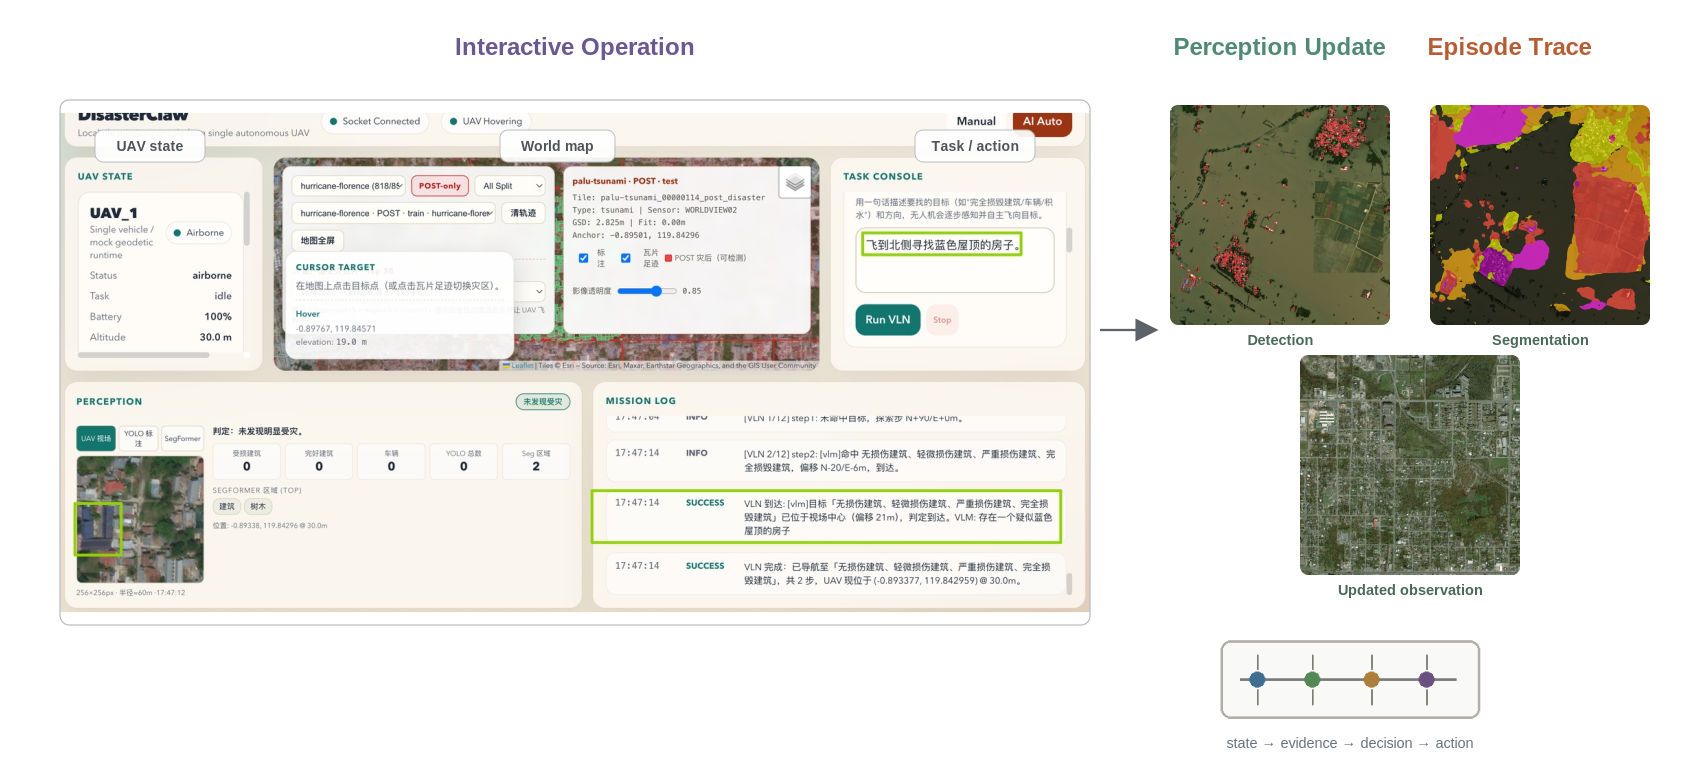
\includegraphics[width=\linewidth]{figure-paper/Fig4_ClosedLoop_Platform.png}
\caption{Representative console, perception displays, and closed-loop instrumentation. This supplied composite shows general platform interfaces, including legacy YOLO/SegFormer and VLN controls; it is not a single synchronized episode or a screenshot of the frozen ChangeOS experiment. The displayed 30 m setting is an interface example, not a height used in the camera-ladder evaluation. Quantitative results use the headless protocol described in Section~\ref{sec:setup}.}
\label{fig:console}
\end{figure}
